\subsection{Favoritliste}
\label{subsec:brug-favoritliste}

Når der bliver tilføjet en opskrift til en brugers favoritliste, så kan denne opskrift findes under ``favoritter'', som kan findes via sidehovedet i toppen af siden. Et eksempel af en kort opskriftsliste under favoritter kan ses på \figref{fig:overblik-favoritter}.

\begin{figure}[H]
	\centering
	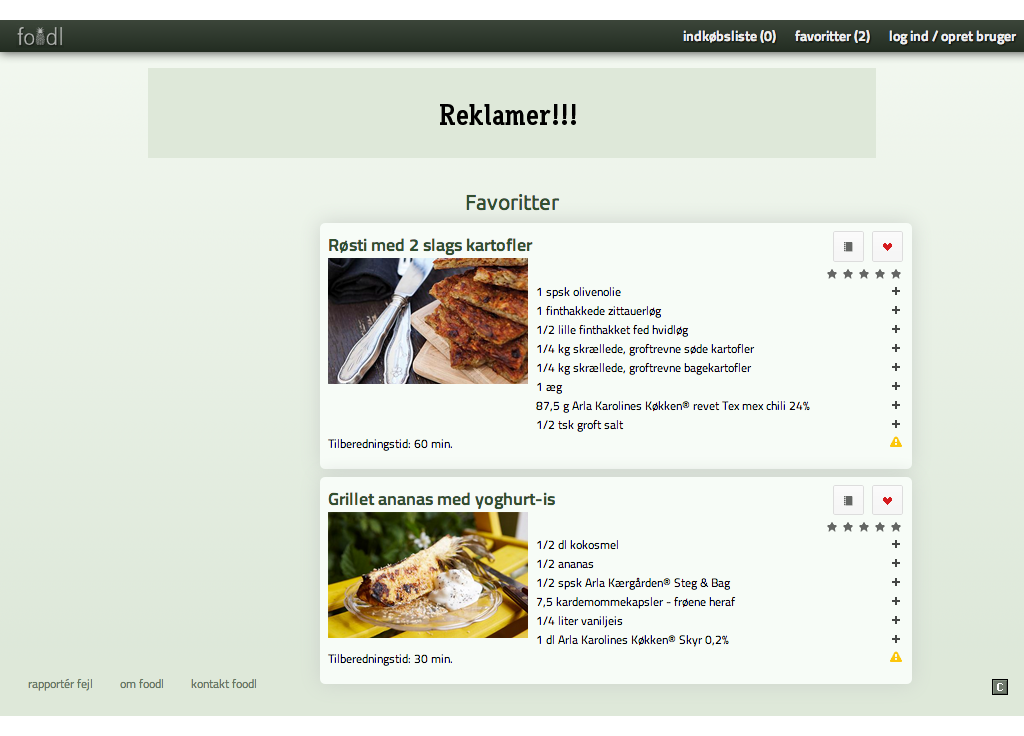
\includegraphics[scale=1]{billeder/foodl/thumbnails/favoritter.png}
	\capt{Denne figur har til formål at give et overblik over systemets favoritside.}
	\label{fig:overblik-favoritter}
\end{figure}

En opskrift bliver tilføjet til favoritlisten ved at trykke på den hjerte-formede knap i øverste højre hjørne af en opskrift. Hvis en opskrift ikke er favoriseret, så er det hjerteformede område i knappen gråt. Når den bliver favoriseret, så bliver hjertet rødt, og dette kan ses i \figref{fig:overblik-favoritter}.

Idéen med favoritlisten er at give brugerne mulighed for at gemme opskrifter, de finder interessante og at de gerne vil bogmærke den til næste gang. De er meget nemmere at finde frem, når man kan finde dem under favoritlisten i stedet for at skulle udføre en ny søgning og prøve at finde den samme opskrift igen.
